%==============================================================

\chapter{Results}\label{bds2}

Very small 100 Song Dataset plus 20 Cover Songs to evaluate and compare similarity metrics. Full similarity matrices. 
High performance/ throughput tests with full 12000 song testset to evaluate full load performance.\\

\section{Runtime}

\section{feature separation quality}\label{featqual}

\textit{\textbf{Which features are useful, which not (looking at you rhythm histogram)\\}}
\\

\noindent skl scaled and unscaled\ref{fig:sklsc}\\
problem with outliers \ref{sparkskl}

\begin{figure}[htbp]
	\centering
	\framebox{\parbox{1\textwidth}{ 
	\begin{subfigure}{0.5\textwidth}
		\centering
		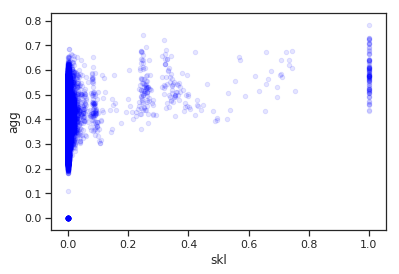
\includegraphics[scale=0.5]{Images/SparkFeat/skl_unscaled.png}
		\captionof{figure}{SKL unscaled}
		\label{scklusc}
	\end{subfigure}
	\begin{subfigure}{0.5\textwidth}
		\centering
		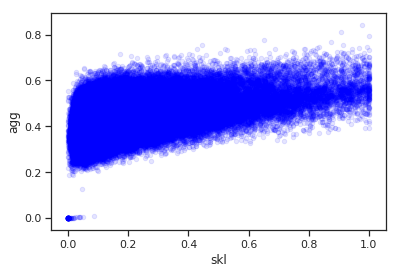
\includegraphics[scale=0.5]{Images/SparkFeat/skl_scaled.png}
		\captionof{figure}{SKL scaled}
		\label{scklsc}
	\end{subfigure}%
	}}
	\caption{Correlation of features}
	\label{fig:sklsc}
\end{figure}

\noindent correlation of features in figure \ref{fig:corr}\\

\begin{figure}[htbp]
	\centering
	\framebox{\parbox{1\textwidth}{
	\begin{subfigure}{0.5\textwidth}
		\centering
		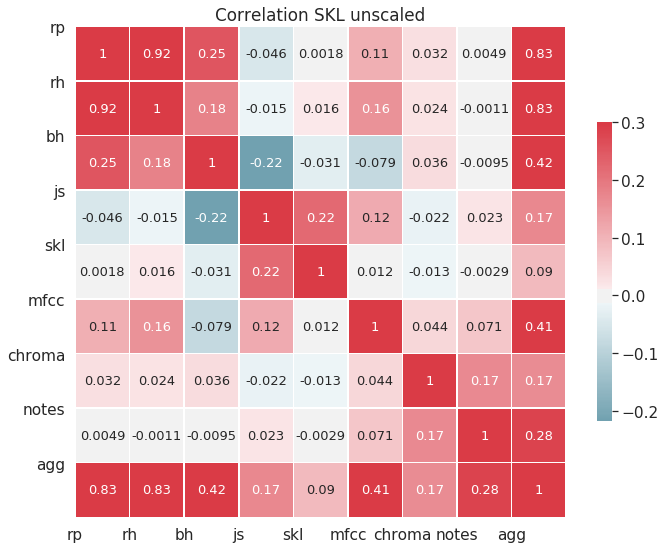
\includegraphics[scale=0.33]{Images/SparkFeat/skl_corr_unscaled.png}
		\captionof{figure}{SKL unscaled}
		\label{corrusc}
	\end{subfigure} 
	\begin{subfigure}{0.5\textwidth}
		\centering
		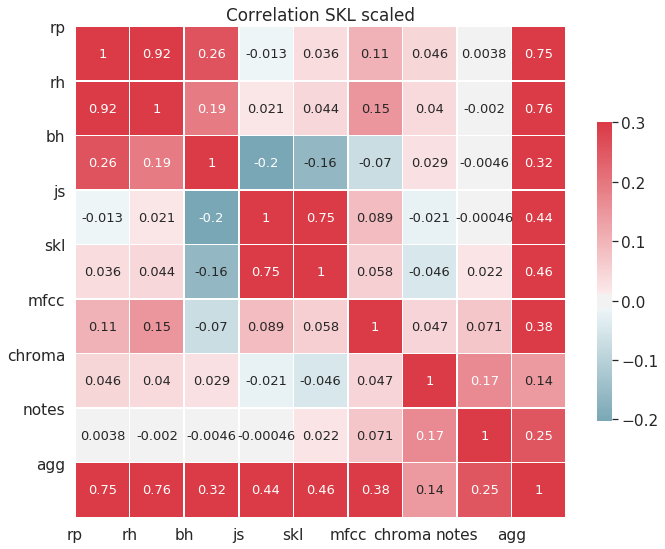
\includegraphics[scale=0.33]{Images/SparkFeat/skl_corr_scaled.png}
		\captionof{figure}{SKL scaled}
		\label{corrsc}
	\end{subfigure}%
	}}
	\caption{Correlation of features}
	\label{fig:corr}
\end{figure}

\begin{figure}[htbp]
	\centering
	\framebox{\parbox{1\textwidth}{ 			
			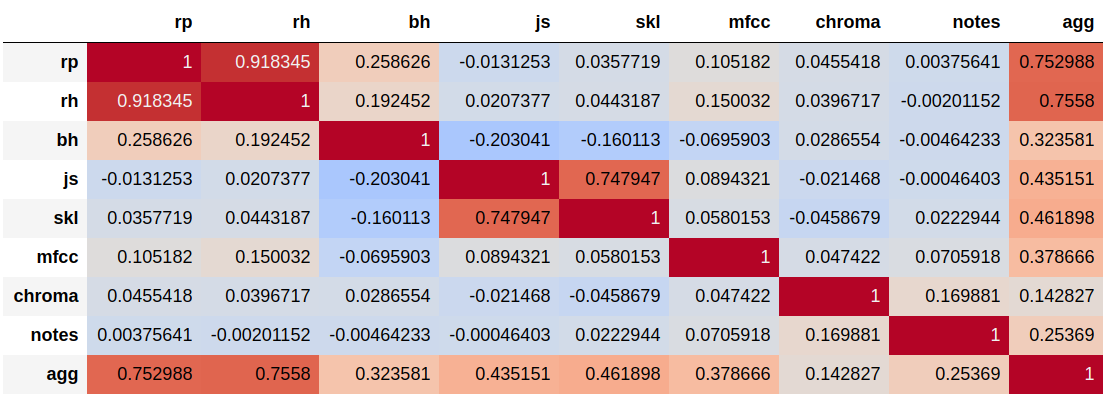
\includegraphics[scale=0.4]{Images/SparkFeat/corr_95_1517.png}	
	}}
	\caption{correlation 95 songs, 19 genres (5 each), 1517 artists}
	\label{fig:corr2}
\end{figure}

\noindent Scatter Matrix, 5 songs of each genre from 1517 artists - distances combined, main diagonal = Kernel Density Estimation in figure \ref{fig:corr3}
\begin{figure}[htbp]
	\centering
	\framebox{\parbox{1\textwidth}{ 			
			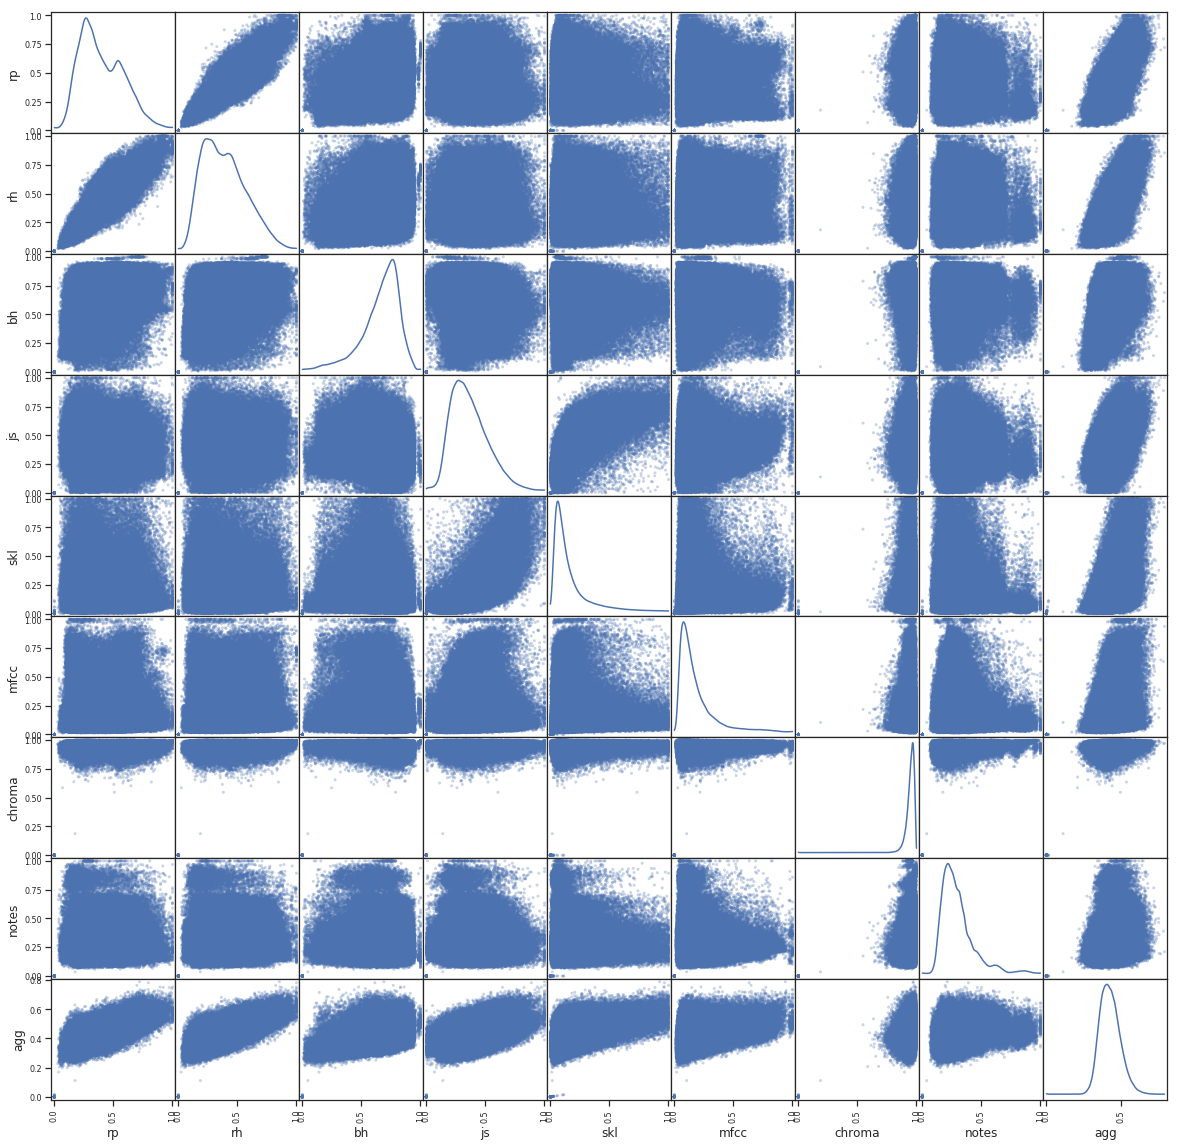
\includegraphics[scale=0.36]{Images/SparkFeat/scatter1517_KernelDensityEstimationHD.png}	
	}}
	\caption{correlation 95 songs, 19 genres (5 each), 1517 artists}
	\label{fig:corr3}
\end{figure}

\noindent Scatter Matrix, 1 Song (Soundtack) from 100 song sample - distances, main diagonal = Kernel Density Estimation, picked subset of 5 genres in figure \ref{fig:corr8}
\begin{figure}[htbp]
	\centering
	\framebox{\parbox{1\textwidth}{ 			
			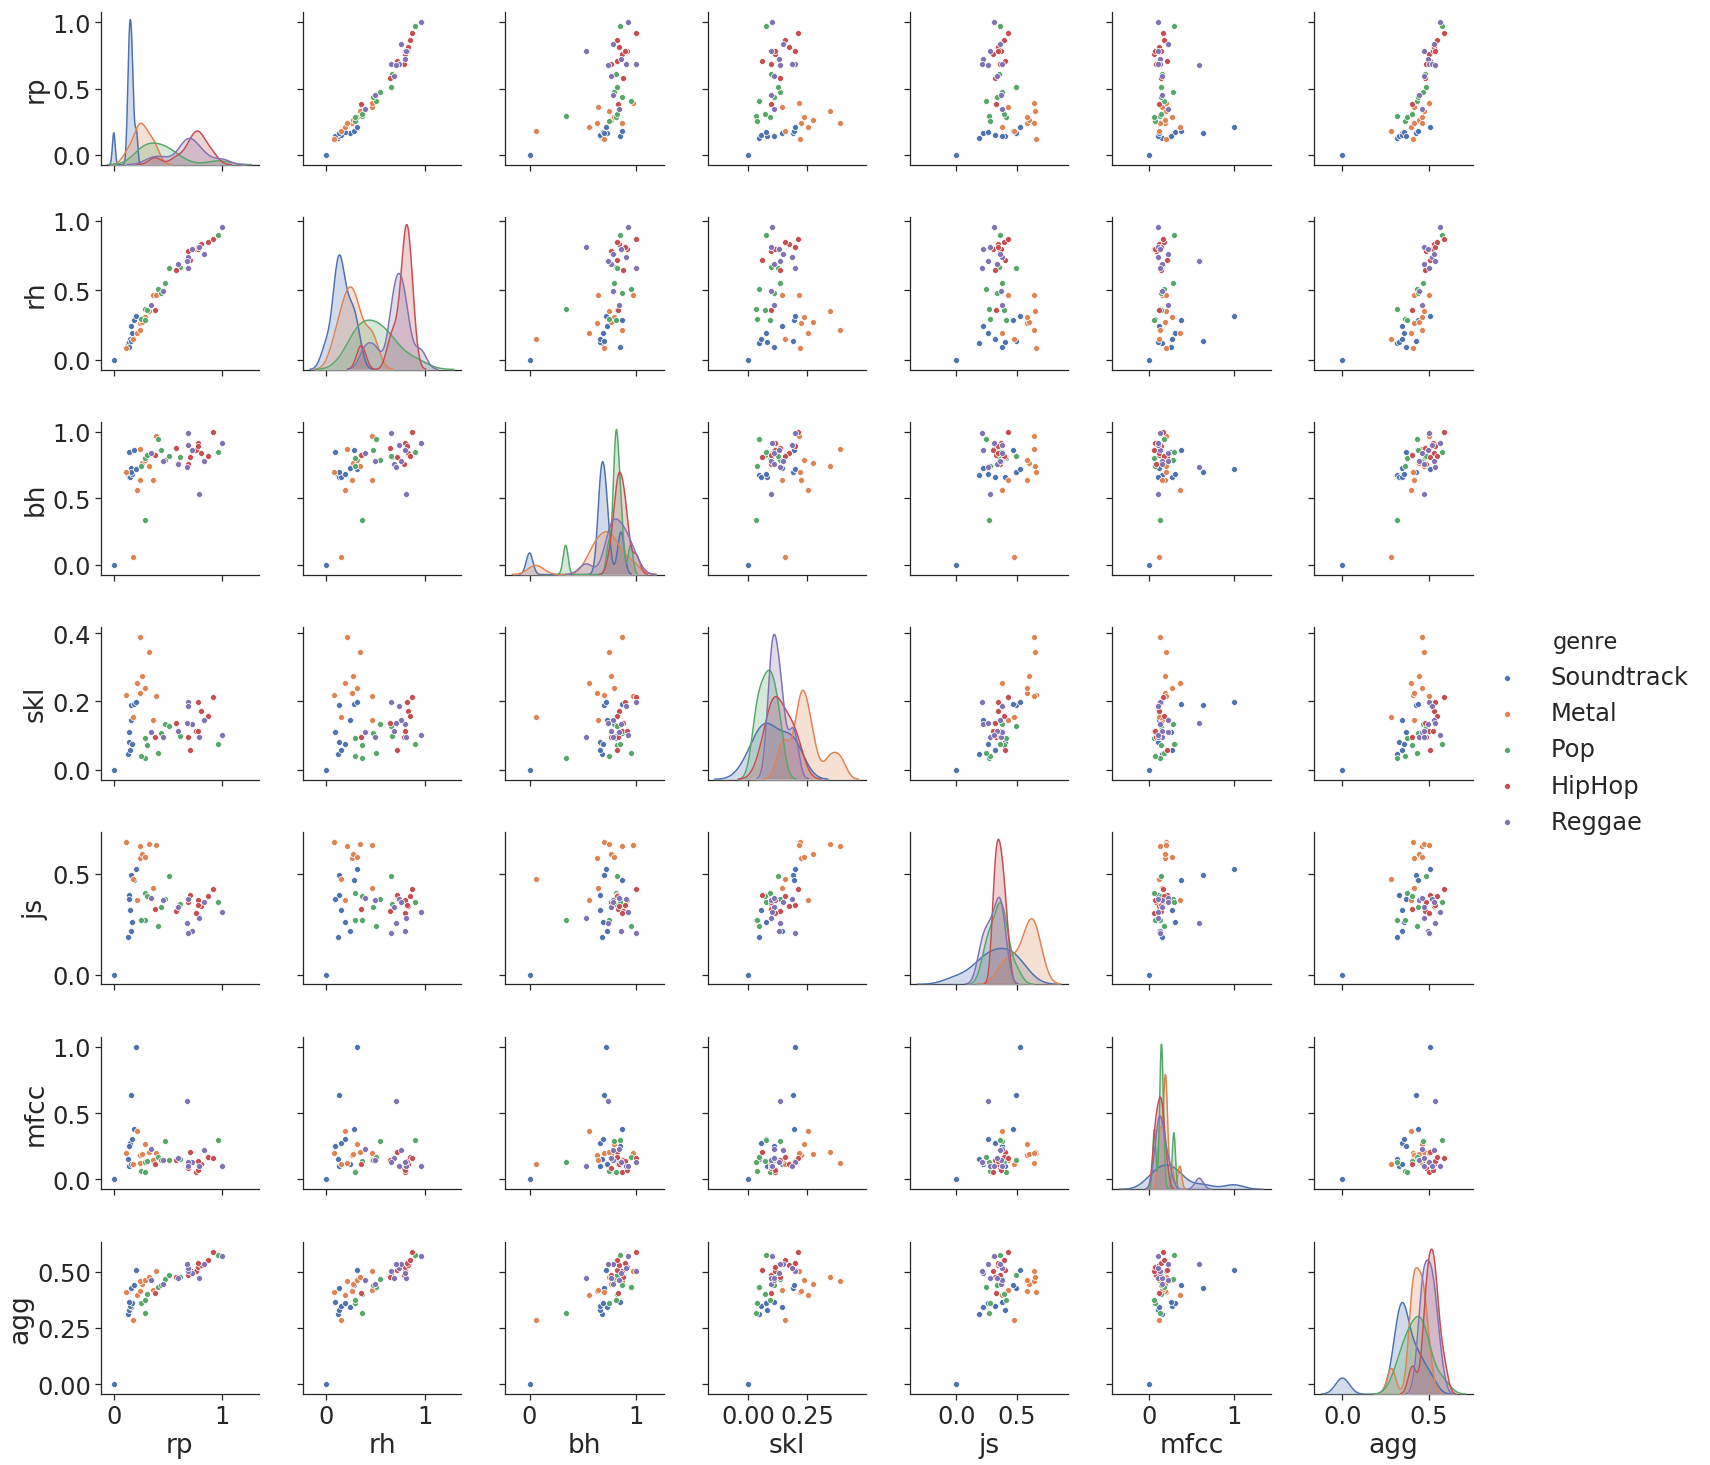
\includegraphics[scale=0.32]{Images/SparkFeat/soundtrack2.png}	
	}}
	\caption{distances 1 song (Soundtrack), 5 genres (10 songs each)}
	\label{fig:corr8}
\end{figure}

\noindent Scatter Matrix, 1 Song (Rock/ Metal) from 1517 artists - distances, main diagonal = Kernel Density Estimation, picked subset of 3 genres\\ All features combined recommends Rock primarily\\
Most interesting Detail: Plot JS - RP: overall similarity JS between Rock and Hip Hop - overall similarity RP between Classical and Metal - only one feature would not be able to separate all 4 genres in figure \ref{fig:corr5}
\begin{figure}[htbp]
	\centering
	\framebox{\parbox{1\textwidth}{ 			
			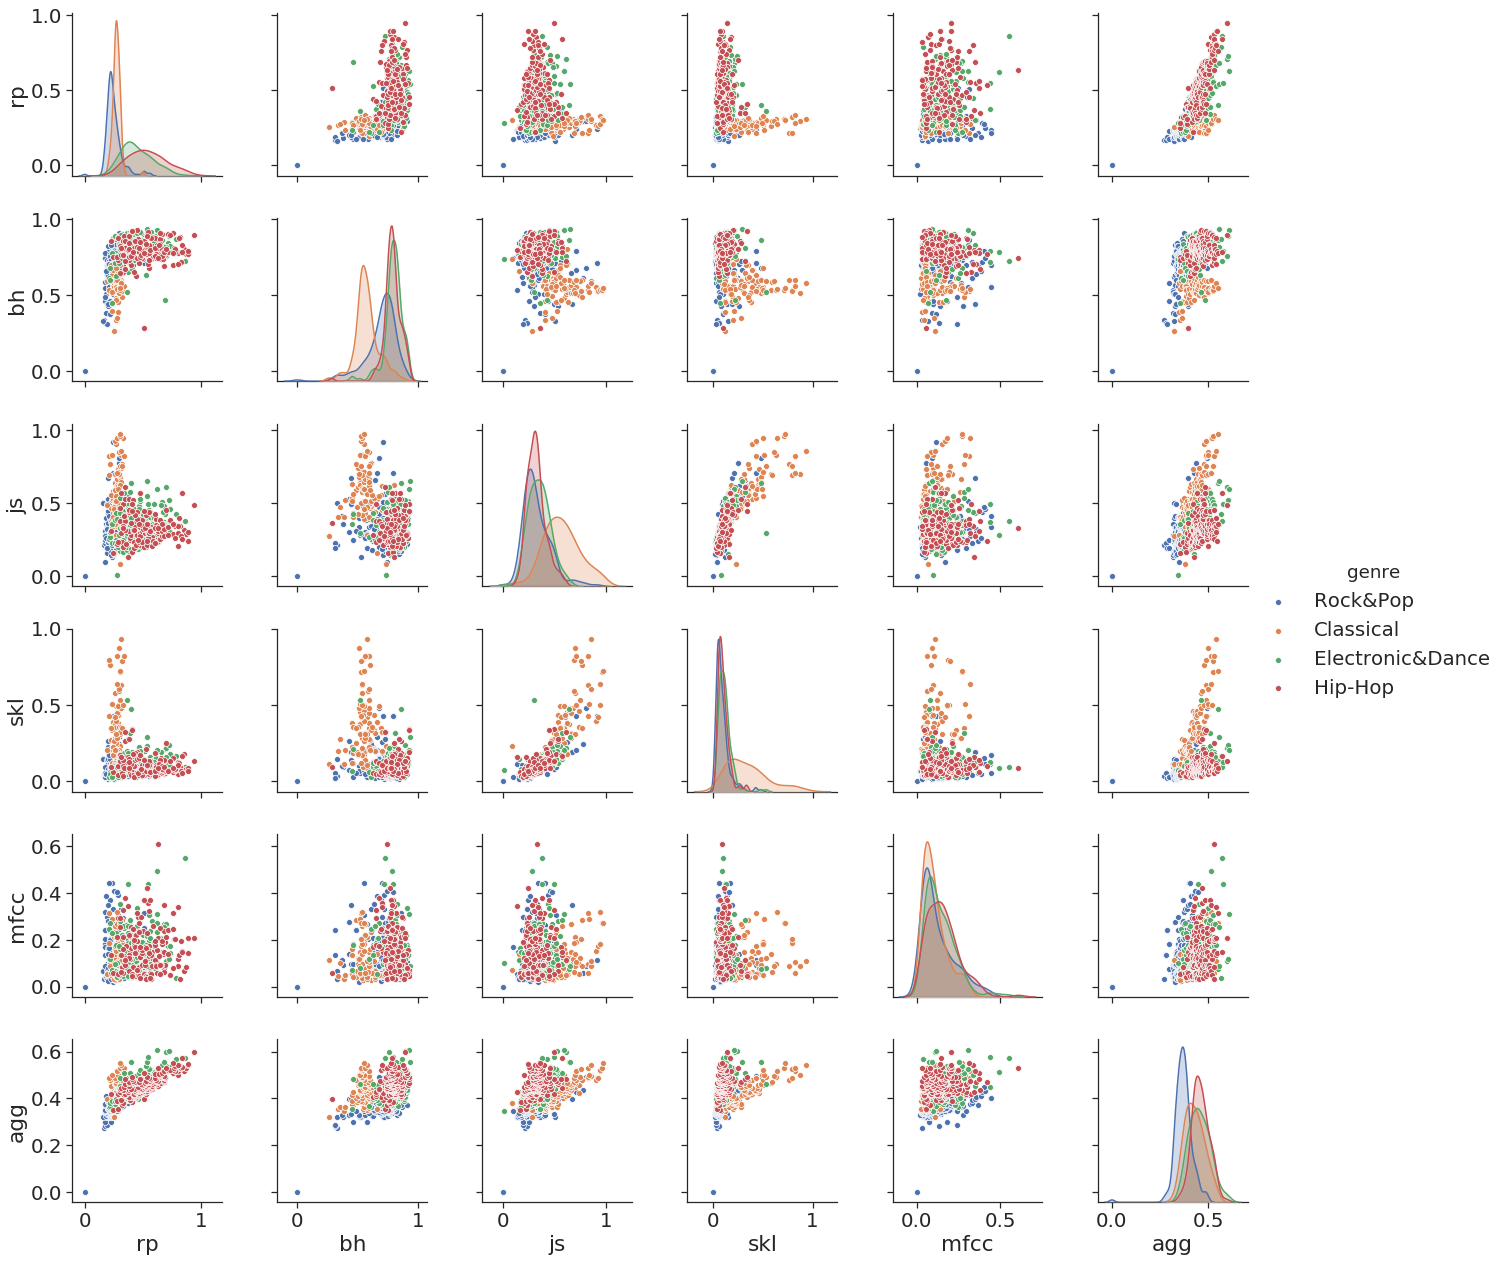
\includegraphics[scale=0.45]{Images/SparkFeat/rock.png}	
	}}
	\caption{distances 1 song, Rock/ Metal, 1517 artists, 4 genres}
	\label{fig:corr5}
\end{figure}

\noindent Scatter Matrix, 1 Song (Electronic) from 1517 artists - distances - figure \ref{fig:corr6}
No combination of features is able to accurately separate HipHop from Rock-Pop
\begin{figure}[htbp]
	\centering
	\framebox{\parbox{1\textwidth}{ 			
			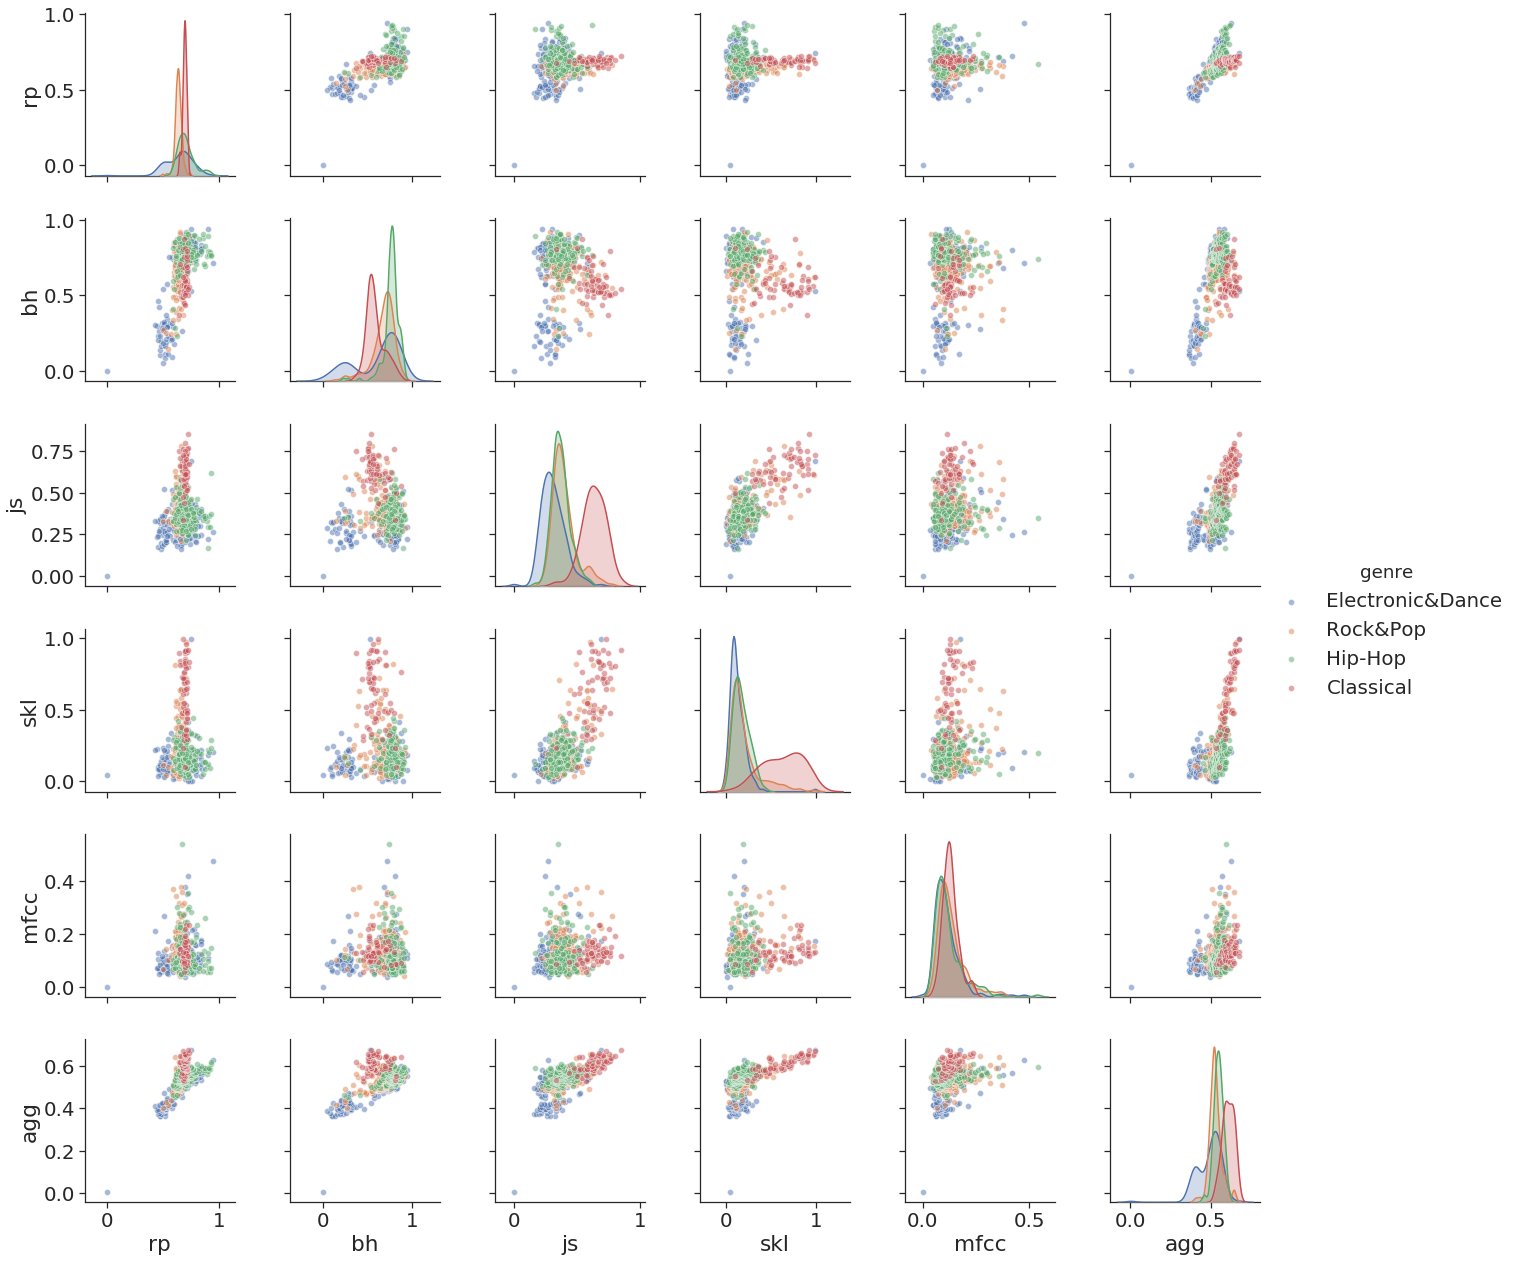
\includegraphics[scale=0.45]{Images/SparkFeat/electronic.png}	
	}}
	\caption{distances 1 song, electronic, 1517 artists, 4 genres}
	\label{fig:corr6}
\end{figure}

\noindent Scatter Matrix, 1 Song (Classics) from 1517 song sample - distances, main diagonal = Kernel Density Estimation, picked subset of 4 genres in figure \ref{fig:corr7}
\begin{figure}[htbp]
	\centering
	\framebox{\parbox{1\textwidth}{ 			
			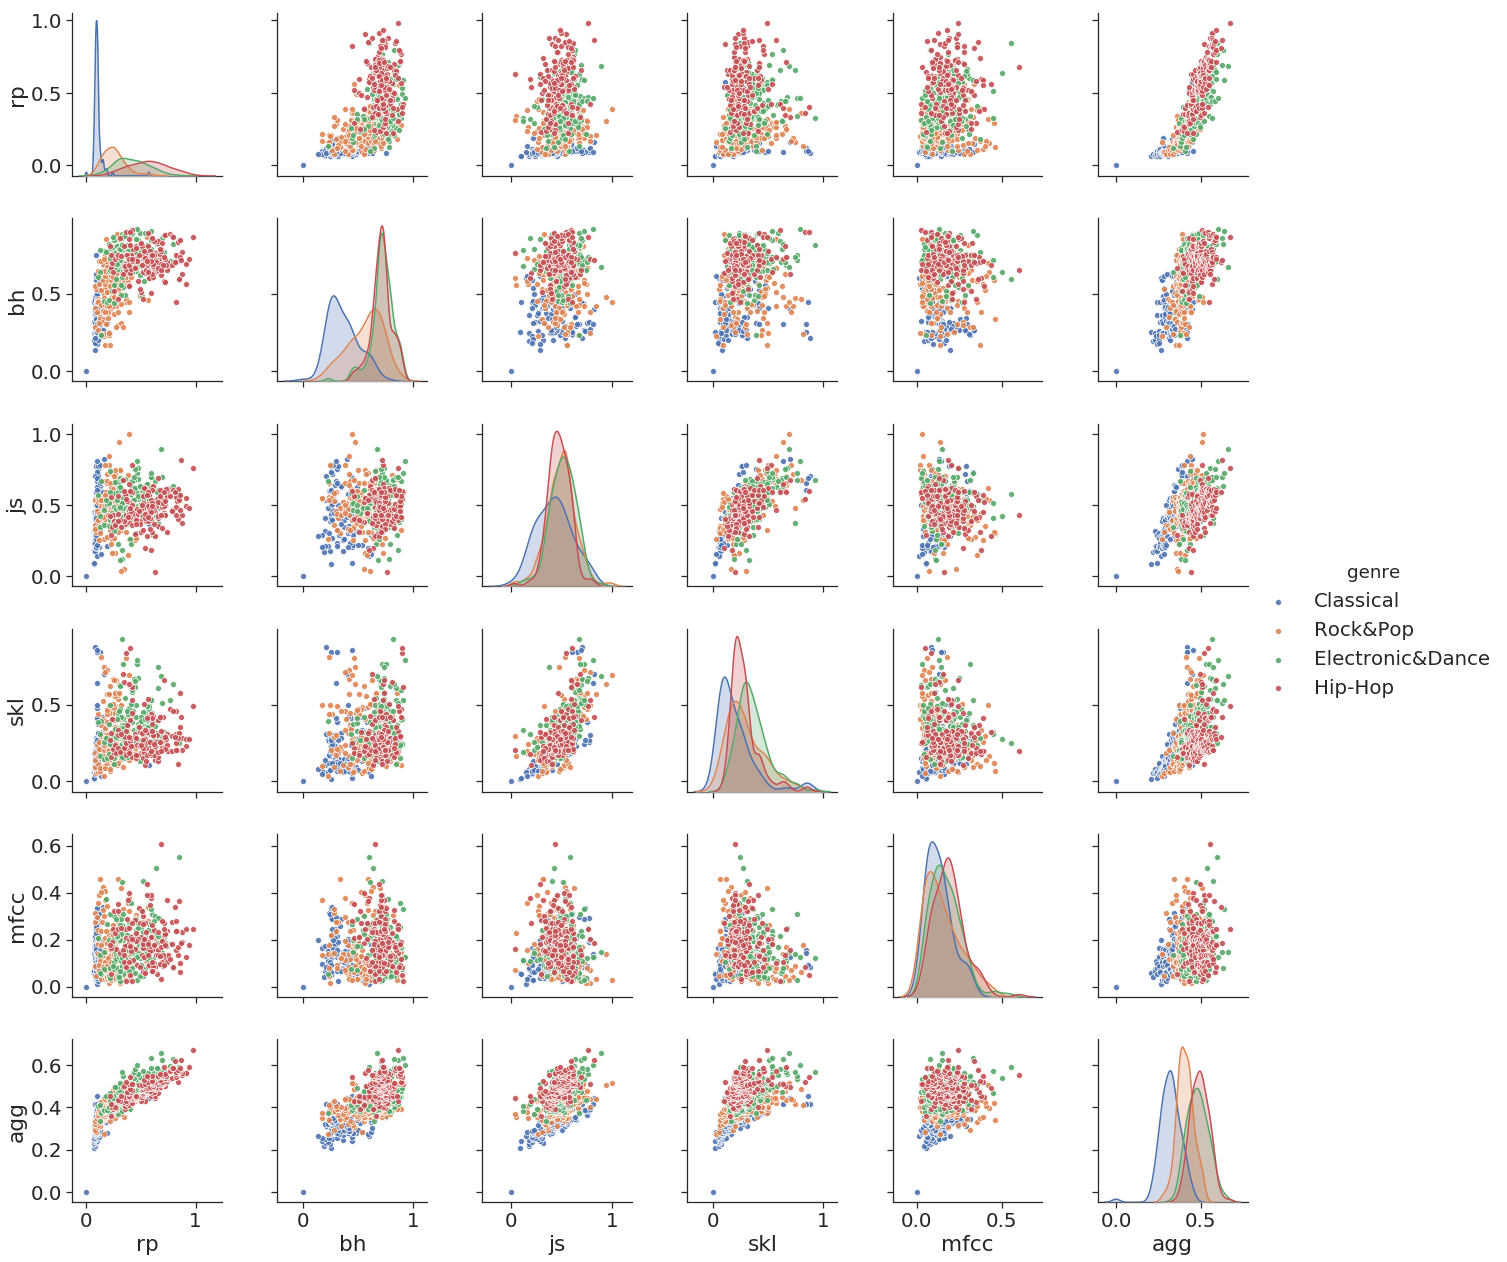
\includegraphics[scale=0.45]{Images/SparkFeat/classical.png}	
	}}
	\caption{distances 1 song (Classical), 4 genres (10 songs each)}
	\label{fig:corr7}
\end{figure}

\noindent distances from classical song out of 1517 artists dataset in figure \ref{fig:featsep}\\

\begin{figure}[htbp]
	\centering
	\framebox{\parbox{1\textwidth}{ 			
			\begin{subfigure}{.495\textwidth}
				\centering    
				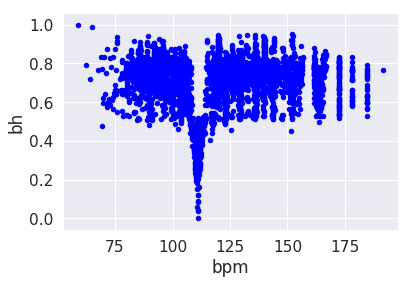
\includegraphics[scale=0.3]{Images/SparkFeat/BH_BPM.png}
				\caption{Beat Histogram vs BPM}
				\label{fs1}
			\end{subfigure}		
			\begin{subfigure}{.495\textwidth}
				\centering     
				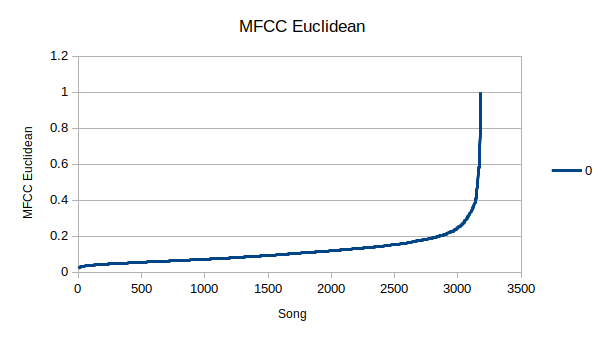
\includegraphics[scale=0.5]{Images/SparkFeat/MFCC_Eucl.png}
				\caption{MFCC Euclidean}
				\label{fs2}
			\end{subfigure}%	
			
			\begin{subfigure}{.495\textwidth}
				\centering    
				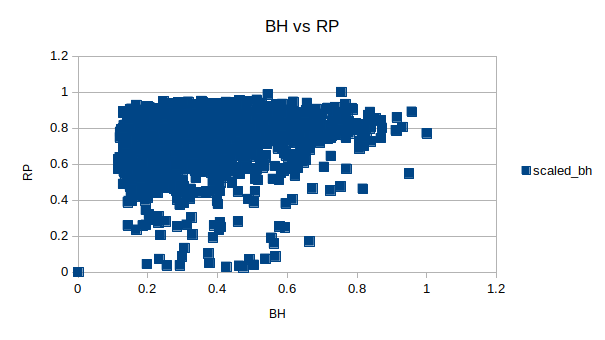
\includegraphics[scale=0.5]{Images/SparkFeat/BH_RP.png}
				\caption{Beat Histogram vs Rhythm Patterns}
				\label{fs3}
			\end{subfigure}
			\begin{subfigure}{.495\textwidth}
				\centering     
				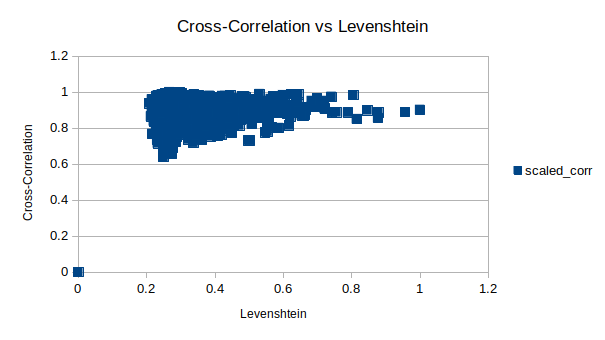
\includegraphics[scale=0.5]{Images/SparkFeat/Cross-Corr_Levenshtein.png}
				\caption{Cross-correlation vs Levenshtein}
				\label{fs4}
			\end{subfigure}%		
	}}
	\caption{genre recall 100 songs}
	\label{fig:featsep}
\end{figure}
\FloatBarrier

\section{Cover song identification}\label{covsongid}

\textit{\textbf{Able to find "Rock you like a Hurricane" cover as top recommendation in over 11500 songs\\}}
\ \\
\textit{\textbf{counting the hits in the top 10 results of 80 requested songs on 164 song dataset covers80:\\}}
\begin{itemize}
	\setlength\itemsep{-0.5em}
	\item chroma + notes + rp: 28
	\item chroma + notes: 24
	\item notes: 24
	\item notes + rp: 22
	\item mfcc + notes + rp: 20 (mfcc faulty)
	\item chroma: 16

\end{itemize}
\textit{interesting sidenote: results of chroma only and notes only different! Nearly ever}

\section{Genre similarity}\label{genrerec}

\textbf{\textit{\underline{100 Song Testset, 10 genres:\\}}} 
\begin{figure}[htbp]
	\centering
	\framebox{\parbox{1\textwidth}{ 			
			\begin{subfigure}{.495\textwidth}
				\centering    
				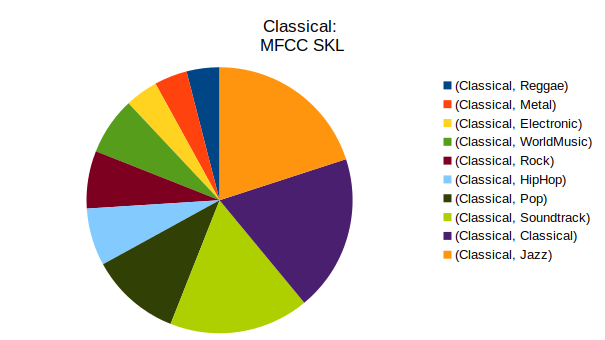
\includegraphics[scale=0.48]{Images/SparkFeat/Classical_MFCC_SKL.png}
				\caption{Classical - MFCC SKL}
				\label{cms}
			\end{subfigure}		
			\begin{subfigure}{.495\textwidth}
				\centering     
				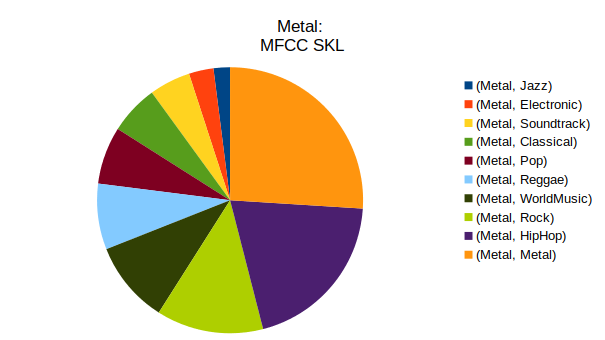
\includegraphics[scale=0.48]{Images/SparkFeat/Metal_MFCC_SKL.png}
				\caption{Metal - MFCC SKL}
				\label{mms}
			\end{subfigure}%	
			
			\begin{subfigure}{.495\textwidth}
				\centering    
				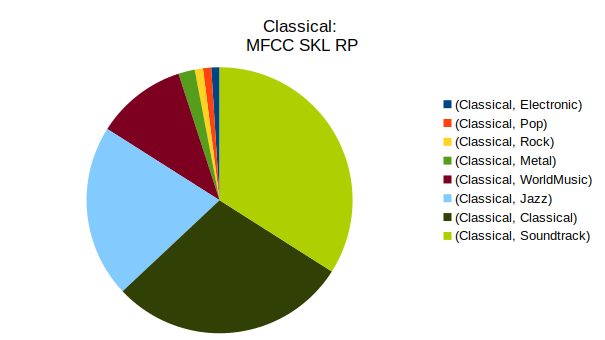
\includegraphics[scale=0.48]{Images/SparkFeat/Classical_MFCC_SKL_RP.png}
				\caption{Classical - MFCC SKL RP}
				\label{cmsr}
			\end{subfigure}
			\begin{subfigure}{.495\textwidth}
				\centering     
				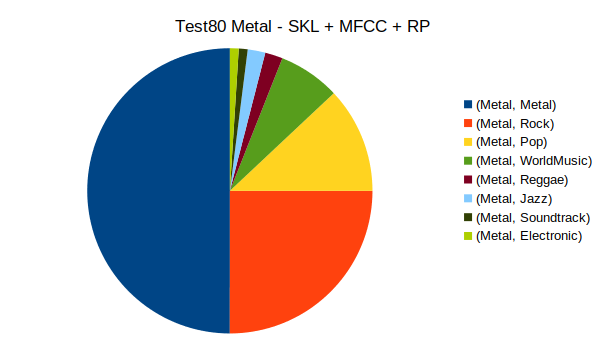
\includegraphics[scale=0.48]{Images/SparkFeat/Metal_MFCC_SKL_RP.png}
				\caption{Metal - MFCC SKL RP}
				\label{mfsr}
			\end{subfigure}%		
	}}
	\caption{genre recall 100 songs}
	\label{fig:genrerec}
\end{figure}


\section{... and beyond genre boundaries}

\textit{\textbf{Rachmaninoff Prelude C\# minor full dataset Top 5 MFCC Euclidean\\}}
\\
Titel: Klassik/Rachmaninoff - Idil Biret - Op 3 No 2 Prelude in C - Sharp Minor
\begin{itemize}
	\setlength\itemsep{-0.5em}
	\item Klassik/Rachmaninoff - Piano Concerto No2 In C Minor Op18-1 Moderato
	\item Klassik/Liszt - Piano Concerto No 1 in E flat major S124(LWH4) Allegro maestoso
	\item Klassik/Brahms - Piano Sonata No2 in F sharp minor Op2 - III Scherzo allegro
	\item \underline{Metal\&Rock/Steve Moore - Intro \& Credits}
	\item Klassik/Liszt - Piano Concerto No 1 in E flat major S124(LWH4) Allegro animato
\end{itemize}

\section{Summary and outlook}

In the first part of this thesis an overview over the field of MIR was given, different audio features were explained, similarity measurements evaluated and multiple algorithms for timbre similarity were presented.\\
Data was collected, over 1TB of music data, 114000 songs. The necessary audio features were extracted and pre-processed (Melody Estimation) in parallel using MPI on a cluster paving the way for usage with big data processing frameworks.\\
The features were loaded into the HDFS of a cluster and multiple similarity measurements were implemented, tested, evaluated and improved. With spark multiple approaches (RDD, DataSet, Filter and Refine, Cluster Configurations) were tested.\\
The results were presented and visualized.\\
\ \\
outlook:\\
\ \\
more state of the art similarity (blocked)\\
performance improvements\\
spark streaming, real-time\\
jensen-shannon investigation\\
Genre and metadata, Genre specific features, combinations and variable model, Collaborative Filtering, Lyrics\\
reduce hubness\\

%\addtolength{\textheight}{-12cm}   % This command serves to balance the column lengths
% on the last page of the document manually. It shortens
% the textheight of the last page by a suitable amount.
% This command does not take effect until the next page
% so it should come on the page before the last. Make
% sure that you do not shorten the textheight too much.